\documentclass[pdf,aspectratio=169]{beamer}
\usepackage[]{hyperref,graphicx,siunitx,lmodern,booktabs}
\usepackage{physics}
\usepackage{em-commands}
\mode<presentation>{\usetheme{EM}}

\graphicspath{ {../Images/} }

\sisetup{per-mode=symbol}

%preamble
\title{Two Roads Diverged\ldots}
\date{August 29, 2018}
\author{Jed Rembold}

\begin{document}
\renewcommand{\theenumi}{\Alph{enumi}}

\begin{frame}{Announcements}
	\begin{itemize}
		\item Homework 1
			\begin{itemize}
				\item Due on Monday night
				\item Please start each problem on a new page
				\item Please when you upload to Gradescope accurately tie which pages correspond to which questions
				\item I'll grade 2 randomly
				\item 14 \emph{cumulative} late days before late = 50\%
			\end{itemize}
		\item Bring your laptop on Friday and make sure it is capable of opening Jupyter notebooks
		\item Friday Reading: Ch 1, Section 4
		\item Question Responses: \href{http://rembold-class.ddns.net}{rembold-class.ddns.net}
	\end{itemize}
\end{frame}

\begin{frame}{}
	The following mathematical operation makes sense and is technically valid.
	\[\nabla \vdot \nabla T(x,y,z) \]
	\begin{enumerate}
		\item Yes, it will produce a vector field
		\item \alert<2>{Yes, it will produce a scalar field}
		\item No, you can't take the divergence of a scalar field
		\item No, but for a completely different reason
	\end{enumerate}

	\pause
	\vspace{5mm}
	What would be the physical significance of this operation? Say I did this operation at some point in space and got a large positive value. What would that indicate?
\end{frame}

\begin{frame}{Interpretations}
	\vspace{-1.5cm}
	\begin{center}
		\includegraphics<1>[width=0.7\textwidth]{scalarfunction.png}
		\includegraphics<2>[width=0.7\textwidth]{gradient.png}
		\includegraphics<3>[width=0.7\textwidth]{divergence.png}
	\end{center}
\end{frame}

\begin{frame}{}
	You are trying to compute the work done by a force, $\force=a\xhat + x\yhat$, along the line $y=2x$ from (0,0) to (1,2). What would be the value of $d\va*{\ell}$?
	\begin{enumerate}
		\item $dx \xhat$
		\item $dy \yhat$
		\item $2dx \xhat$
		\item \alert<2>{Something else}
	\end{enumerate}
\end{frame}

\begin{frame}{}
	You are \emph{still} trying to compute the work done by a force, $\force=a\xhat + x\yhat$, along the line $y=2x$ from (0,0) to (1,2). Which of the following forms of the integral would be correct?
	\[1.\,\,\int_0^1 a\,dx + \int_0^2 x\,dy \qquad 2.\,\,\int_0^1 (a\,dx + 2x\, dx), \qquad 3.\,\, \frac{1}{2}\int_0^2(a\,dy + y\,dy)\]
	\begin{enumerate}
		\item Both 1 and 2
		\item \alert<2>{Both 2 and 3}
		\item Both 1 and 3
		\item All 3 are correct
	\end{enumerate}
\end{frame}

\begin{frame}{}
	Suppose a fluid has a velocity field given by $\va{v} = x\xhat + z\yhat$. Which components of the field contribute to the "fluid flux" integral ($\int_S \va{v}\vdot d\va{A}$) through the x-z plane?
	\begin{enumerate}
		\item $v_x$
		\item \alert<2>{$v_y$}
		\item Both contribute
		\item Neither contribute
	\end{enumerate}
\end{frame}

\begin{frame}{}
	Consider the same fluid with velocity field of $\va{v} = x\xhat + z\yhat$. What is the value of the fluid flux integral ($\int_S \va{v}\vdot d\va{A}$) through the \emph{entire} x-y plane?
	\begin{enumerate}
		\item \alert<2>{It is zero}
		\item It is something finite
		\item It is infinite
		\item I don't have time to do this integral
	\end{enumerate}
\end{frame}

\begin{frame}{}
	Evaluate the following line integral where $T(x,y) = xy+\frac{5}{x}$:
	\[\int_{(1,2)}^{(5,1)} (\grad T)\vdot d\va*{\ell} \]
	\begin{enumerate}
		\item -26
		\item \alert<2>{-1}
		\item 20
		\item I can't solve this without knowing a path
	\end{enumerate}
\end{frame}

\begin{frame}{}
	Which of the following two fields has zero divergence?
	\begin{center}
		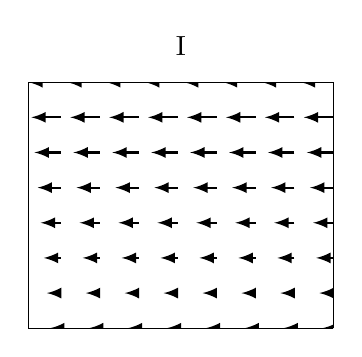
\begin{tikzpicture}
			\begin{axis}[
				domain = 1:3,
				title = I,
				view = {0}{90},
				samples = 8,
				ticks = none,
				width=.45\textwidth,
				]
				\addplot3[thick, quiver={u={-y}, v={0}, scale arrows=0.08}, -latex] (x,y,0);
				
			\end{axis}
		\end{tikzpicture}\hspace{1cm}
		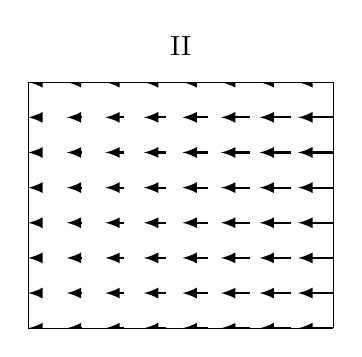
\begin{tikzpicture}
			\begin{axis}[
				domain = 1:3,
				title = II,
				view = {0}{90},
				samples = 8,
				ticks = none,
				width=.45\textwidth,
				]
				\addplot3[thick, quiver={u={-x}, v={0}, scale arrows=0.08}, -latex] (x,y,0);
			\end{axis}
		\end{tikzpicture}
		\begin{enumerate}
			\item Both do
			\item \alert<2>{Only I is zero}
			\item Only II is zero
			\item Neither is zero
		\end{enumerate}
	\end{center}
\end{frame}

\begin{frame}{}
	Which of the following two fields has zero curl?
	\begin{center}
		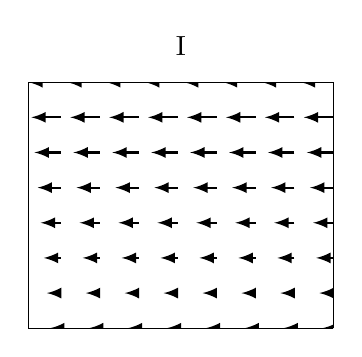
\begin{tikzpicture}
			\begin{axis}[
				domain = 1:3,
				title = I,
				view = {0}{90},
				samples = 8,
				ticks = none,
				width=.45\textwidth,
				]
				\addplot3[thick, quiver={u={-y}, v={0}, scale arrows=0.08}, -latex] (x,y,0);
				
			\end{axis}
		\end{tikzpicture}\hspace{1cm}
		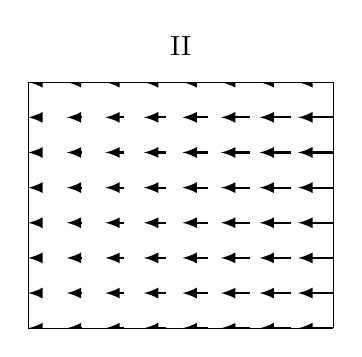
\begin{tikzpicture}
			\begin{axis}[
				domain = 1:3,
				title = II,
				view = {0}{90},
				samples = 8,
				ticks = none,
				width=.45\textwidth,
				]
				\addplot3[thick, quiver={u={-x}, v={0}, scale arrows=0.08}, -latex] (x,y,0);
			\end{axis}
		\end{tikzpicture}
		\begin{enumerate}
			\item Both do
			\item Only I is zero
			\item \alert<2>{Only II is zero}
			\item Neither is zero
		\end{enumerate}
	\end{center}
\end{frame}
\end{document}
